In this section we present formal foundations the MDE framework required for the problem of model search.
The concepts in this section are primerily distilled from the Object Managament Group's Meta-Object Facility.

%%%%%%%%%%%%
% Model
%%%%%%%%%%%%
\subsection{Object Models}
At the center of Model Driven Engineering is the concept of \textit{model}.
Models represent \textit{systems under study}.
This relation between model and system under study, is named \textit{represents} and is given the symbol $\mu$.

\begin{figure}[h]
    \centering
    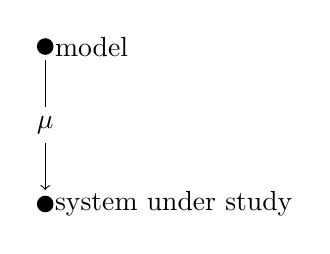
\begin{tikzpicture}
        \coordinate [label=0:{system under study}] (M) at (0,0);
        \coordinate [label=0:{model}]  (MM) at (0,2);
      
          \fill (M) circle (3pt);
          \fill (MM) circle (3pt);
          
        \draw[->, shorten <= 5pt, shorten >= 5pt,] (MM) -- (M) node [midway,fill=white] {$\mu$};
    \end{tikzpicture}
    \caption{$\mu$: \textit{a model represents a system under study}}
\end{figure}

Models often represent only part of the system under study, especially when the system under study is very complex.

\subsubsection{Definitions}

\noindent
\textbf{Object}: 
an object is an entity that identifies information.
Objects can represent things from the real world, or abstract concepts.
Objects are uniquely identifiable.
Objects can be associated, composed or otherwise linked.
For instance, an object can be used to represent a person: with properties such as their name or age, or their links to other people.

\noindent
\textbf{Object Property}: a named collection of elements, representing information from the system under study.
Depending on the type of elements, a property is either an attribute or a reference.

\noindent
\textbf{Property Access}: the process of access the information indentified by an object.
These kind of functions are often called \textit{getters} and \textit{setters}:
$$get(o,p) : \inlineocl{Object}\times\inlineocl{Property} \rightarrow \inlineocl{Collection}$$
$$set(o,p,c) : \inlineocl{Object}\times\inlineocl{Property}\times\inlineocl{Collection} \rightarrow \emptyset$$

\noindent
\textbf{Object Model}: (or simply \textbf{model} throught this thesis) is a set of object that maybe linked to one another. 
Such models can also be described as directed multigraphs $G=\tuple{V,E}$, where the verticies $V$ are associated with objects and the edges $E$ with the links between them.
MOF provides a specification for the serialization of Object Models based on XML called XMI.

% \subsubsection{General Example using XML}
% \begin{listing}[!h]
%     \begin{lstlisting}[language=xml]
%     <Model>  
%         <object att="information one" ref="//@object.1"/>
%         <object att="information two" ref="//@object.0"/>
%     </Model>
%     \end{lstlisting}
%     \caption{Minimal Object Model in the XMI-like format}
% \end{listing}
% In this listing we see a simple model, with two linked objects, each object holds some information.
% It is specified in an XML-like markup language called XML Metadata Interchange.
% XMI is the standard for serialising MOF models.


\subsubsection{Simple Example : Family Tree}
\begin{figure}[!h]
    \centering
    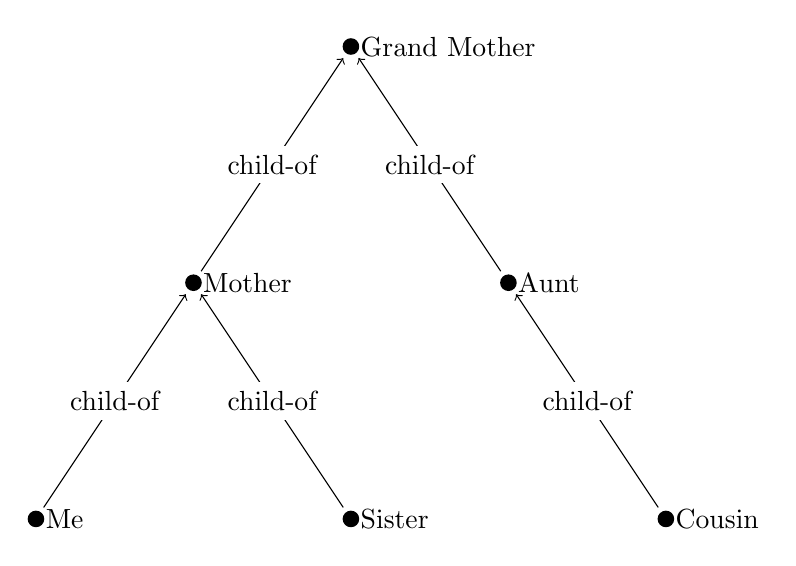
\begin{tikzpicture}
    \coordinate [label=0:{Grand Mother}] (GM) at (4,6);
    \coordinate [label=0:{Mother}] (M) at (2,3);
    \coordinate [label=0:{Aunt}] (A) at (6,3);
    \coordinate [label=0:{Me}] (X) at (0,0);
    \coordinate [label=0:{Sister}] (S) at (4,0);
    \coordinate [label=0:{Cousin}] (C) at (8,0);

    \fill (GM) circle (3pt);
    \fill (M) circle (3pt);
    \fill (A) circle (3pt);
    \fill (X) circle (3pt);
    \fill (S) circle (3pt);
    \fill (C) circle (3pt);

    \draw[->, shorten <= 5pt, shorten >= 5pt,] (M) -- (GM) node [midway,fill=white] {child-of};
    \draw[->, shorten <= 5pt, shorten >= 5pt,] (A) -- (GM) node [midway,fill=white] {child-of};
    \draw[->, shorten <= 5pt, shorten >= 5pt,] (X) -- (M) node [midway,fill=white] {child-of};
    \draw[->, shorten <= 5pt, shorten >= 5pt,] (S) -- (M) node [midway,fill=white] {child-of};
    \draw[->, shorten <= 5pt, shorten >= 5pt,] (C) -- (A) node [midway,fill=white] {child-of};
    \end{tikzpicture}
\caption{\textbf{Simple family tree}: a basic hierarchical representation.}
\end{figure}
An illustrative example for models as graphs are family trees.
A family tree represents people and their familial connections.   
Each node of a family tree corresponds to a person, and is labeled with their name.
Each vertex is an instance of the relation \textit{is a child of}.

\begin{figure}[!h]
    \centering
    \begin{tikzpicture}[level distance=15mm,
        every node/.style={font=\small},
        level 1/.style={sibling distance=45mm},
        level 2/.style={sibling distance=25mm}]
      \node (S) {S}                              % Sentence
        child {node (NP) {NP}                   % Noun Phrase
          child {node (Det) {Det}
            child {node {this}}}}
        child {node (VP) {VP}                   % Verb Phrase
          child {node (V) {V}
            child {node {is}}}
          child {node (NP2) {NP}
            child {node (Det2) {Det}
              child {node {an}}}
            child {node (N) {N}
              child {node {expression}}}}};
      \end{tikzpicture}      
\caption{Syntatic Tree of \textit{this is an expression}}
\end{figure}
Being able to model expressions and languages is a powerful and fundamental feature of object models.
This graph describes the structure of the expression: \textit{this is an expression}.
Here objects represent syntatic structures, such as N noun, Det determinents, V verb, NP noun phrase, and VP verb phrase.
Here we have two NP, one composde of only a Det, and another composed of a Det followed by a N.

\begin{figure}[!h]
  \centering
  \begin{tikzpicture}[level distance=15mm,
      every node/.style={font=\small},
      level 1/.style={sibling distance=35mm},
      level 2/.style={sibling distance=25mm}]
    \node (E) {=}                              % Root: equals expression
      child {node (ADD) {+}                   % Addition subtree
        child {node (NUM1) {2}}
        child {node (NUM2) {2}}}
      child {node (NUM3) {4}};                % Result
  \end{tikzpicture}
\caption{AST of the expression \textit{2 + 2 = 4}}
\end{figure}
Formal languages are commonly manipulated as Abstract Syntax Trees.
In this figure we see the AST for the expression: \textit{2 + 2 = 4}. 
Here the objects correspond to the different symbols of the expression, and the links show how the symbols are organised.





%%%%%%%%%%%%
% Metamodels
%%%%%%%%%%%%
\subsection{Metamodels}
Metamodels are arguably the most important type of model for model driven engineering.
A metamodel is a model that represents a set of models.
A model from that set is said to \textit{conform to} the metamodel.

\begin{figure}[!h]
    \centering
    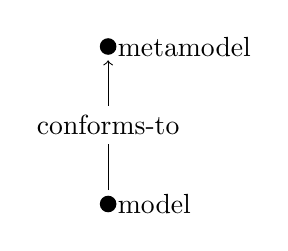
\begin{tikzpicture}
        \coordinate [label=0:{model}] (M) at (0,0);
        \coordinate [label=0:{metamodel}]  (MM) at (0,2);
      
          \fill (M) circle (3pt);
          \fill (MM) circle (3pt);
          
        \draw[->, shorten <= 5pt, shorten >= 5pt,] (M) -- (MM) node [midway,fill=white] {conforms-to};
    \end{tikzpicture}
    \caption{\textit{a model conforms to a metamodel}}
\end{figure}


Metamodels can be formalised with many different languages.
This current section is a simplified metamodel for object and class based modeling, and the following sections are summaries of the UML and OCL metamodels.
For our use-cases, metamodels will come in two parts: 
a collection of class specifications,
and model constraints.
Class specifications define the classes of objects that can be used to make a model 
and define for each class their properties: their attributes and their relations.
Model constraints are use to limit the combinations of objects and the values of their properties.
Model constraints therefore rely on language to query the model.

\subsubsection{Definitions}

\noindent
\textbf{Metamodel}: A metamodel is a tuple $\tuple{M,C}$ where $M$ is a classification model and $C$ is a set of model constraints.

\noindent
\textbf{Conformity}: A model which conforms to a metamodel.

\noindent
\textbf{Classification Model}: Classification models, are a set of classes that maybe be linked to one another.
They are object models representing classification systems: their objects called classes and take a specific form.
% The types of objects in a model conforming to a metamodel are specified in the classification model.
% The types of objects and links are specified in the classification model.

\noindent
\textbf{Class}: Classes represent sets of object, naming them and listing their properties.
For instance, a class can represent and name the concept of a \textit{person}, objects representing people are part of the set the class represents.
The list of properties describe the form objects can take in conforming models.
Classes come in the form of named list of property specifications.
% $$\inlineumlclass{CLASS\_NAME}{\dots}$$

\noindent
\textbf{Property}: a name, type, and collection cardinality.
They specify the information that can be associated with objects.
% $$\inlineumlprop{PROPERTY\_NAME}{TYPE}{m}{n}$$

\noindent
\textbf{Attribute}: named collection of integers associated to an object.

\noindent
\textbf{Reference}: named collection of objects of the model linked to an object.

\noindent
\textbf{Model Constraint}: a constraint expression identifying objects and stating invariants about their combinations or the combination of their properties.
Model constraints are expressions which predicate on the structure of models conforming to the metamodel.
These expressions rely on the vocabulary introduced by the classes and their properties.
Model constraint languages may also provide syntax to navigate a model  

\noindent
\textbf{Meta-Metamodel}:
Metamodels can also be an element of the set they represent, meaning they conform to themselves.
Metamodels can conform to meta-metamodels.

Using the intuition of metamodels as languages: Using the English language, we can describe the English language.

\noindent
\textbf{Domain Specific Language}: 
Domain specific languages are a practical and powerful application of metamodeling.
A powerful intuition for metamodels is that of \textit{metamodels are languages}.
This sentence is an expression which conforms to the vocabulary and the grammar of the English language.
English can be described as a set of words (or bits of words), and rules to combine them.
Expressions in English can represent parts of the real world or abstract ideas.
Domain specific languages leverage this equivalence between metamodels and languages, and use metamodeling frameworks to assist in their development. 
In contrast to general purpose languages (GPL), such as C++, python and Java, DSLs are less expressive but simpler for their given domain.


\subsubsection{Simple Examples of inline notation}
Through out the thesis we'll use inline notation for simple models.
As described above, classes often take the form of named lists of properties.
Taking inspiration from C-like languages, we first name the class, then list the properties between brackets: 
$$\inlineumlclass{CLASS\_NAME}{\dots}$$
Properties are named collections of at least m and at most n elements, of which the elements are typed:
$$\inlineumlprop{PROPERTY\_NAME}{TYPE}{m}{n}$$
Type in our notation is similarly taken from UML standard: \inlineocl(:Type).
Cardinality is noted using intervals: \inlineocl{[m,n]}, where m is minimum cardinality, and n maximum cardinality.

$$\inlineumlclass{Object}{\inlineumlprop{att}{Int}{m}{n}, \inlineumlprop{ref}{Object}{m'}{n'}}$$
This simple metamodel show the general shape of metamodels.
Here we have one class named \inlineocl{Object} representing \textit{objects}.
This class lists two properties: \inlineocl{att} an attribute, and \inelineocl{ref} a reference to other objects in the \inlineocl{Object} class.
Properties being collections, this metamodel also specifies their minimum \inlineocl{m} and maximum \inlineocl{n} number of elements.

$$\inlineumlclass{Person}{\inlineumlprop{age}{Int}{1}{1}, \inlineumlprop{children}{Person}{0}{*}}$$
$$\forall p,q \in \texttt{Person}, p \in q\texttt{.children} \implies p\texttt{.age} < q\texttt{.age}$$
This simple metamodel desribes the person object we've used in previous examples.

% $$\inlineumlclass{Expression}{\inlineumlprop{value}{Int}{1}{1}, \inlineumlprop{subexp}{Expression}{0}{*}}$$
% $$\inlineumlclass{Addition extends Expression}{}$$
% $$\inlineumlclass{Variable extends Expression}{}$$
% $$\forall a\in \texttt{Addition}, |aq\texttt{.subexp}|=2 \wedge a\texttt{.value}= a.q\texttt{.subexp}$$
% This simple metamodel for summation expressions such as $3+4+2$.

%%%%%%%%%%%%
% Model Transformation
%%%%%%%%%%%%
\subsection{Model Validation and Transformation}

% \subsubsection{Model Validation}
\noindent
\textbf{Model Validation}: the process of checking a model conforms to a metamodel.
Models can have errors, because of this modeling tools generally provide a means to leverage the metamodel to check for them.


% \subsubsection{Model Transformation}
\noindent
\textbf{Model Transformation}: 
Model Transformation is the core operation on models.
Model Transformation refers to both the process of transforming models to conform to a new metamodel, and the model of the process.
Model Transformation Execution, generates a target model from a source model according to the MTspec.
Model Transformation Specifications, link classes and properties across metamodels, written in a Model Transformation Language.
Model Transformation Language, generally a super-set of a model constraint language, using query expressions to connect properties and classes.

\begin{figure}[h]
    \centering
    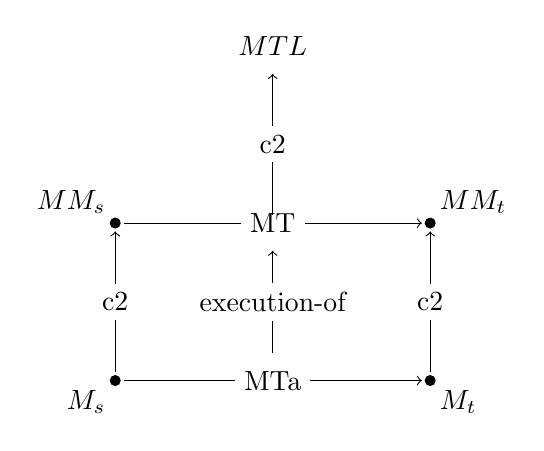
\begin{tikzpicture}
        \coordinate [label=-100:{$M_s$}]  (SM) at (0,0);
        \coordinate [label=-80:{$M_t$}] (TM) at (4,0);
        \coordinate (M2M) at (2,0);
        
        \coordinate [label=100:{$MM_s$}]  (SMM) at (0,2);
        \coordinate [label=80:{$MM_t$}]  (TMM) at (4,2);
        \coordinate (MM2MM) at (2,2);

        \coordinate [label=90:{$MTL$}] (TLMM) at (2,4);
        
            \fill (SM) circle (2pt);
            \fill (TM) circle (2pt);
            \fill (SMM) circle (2pt);
            \fill (TMM) circle (2pt);
        
        \draw[->, shorten <= 3pt, shorten >= 3pt] (SM) -- (TM) node [midway,fill=white] {MTa};
        \draw[->, shorten <= 3pt, shorten >= 3pt] (SMM) -- (TMM) node [midway,fill=white] {MT};
        \draw[->, shorten <= 3pt, shorten >= 3pt,] (SM) -- (SMM) node [midway,fill=white] {c2};
        \draw[->, shorten <= 3pt, shorten >= 3pt] (TM) -- (TMM)node [midway,fill=white] {c2};
        \draw[->, shorten <= 3pt, shorten >= 3pt] (MM2MM) -- (TLMM)node [midway,fill=white] {c2};

        \draw[->, shorten <= 10pt, shorten >= 10pt,] (M2M) -- (MM2MM) node [midway,fill=white] {execution-of};
    \end{tikzpicture}
    \caption{Transformation Pattern}
\end{figure}

A notable group of model transformations includes those which generate code in a programming language.
From a UML Class Diagram, one can generate a Java Class Specification.